\documentclass[a4paper,12pt]{article} % тип документа

% Поля страниц
\usepackage[left=2.5cm,right=2.5cm,
    top=2cm,bottom=2cm,bindingoffset=0cm]{geometry}
    
%Пакет дял таблиц   
\usepackage{multirow} 
    
%Отступ после заголовка    
\usepackage{indentfirst}


% Рисунки
\usepackage{floatrow,graphicx,calc}
\usepackage{wrapfig}

%%% Работа с картинками
\usepackage{graphicx}  % Для вставки рисунков
\graphicspath{{images/}{images2/}}  % папки с картинками
\setlength\fboxsep{3pt} % Отступ рамки \fbox{} от рисунка
\setlength\fboxrule{1pt} % Толщина линий рамки \fbox{}
\usepackage{wrapfig} % Обтекание рисунков и таблиц текстом

% Создаёем новый разделитель
\DeclareFloatSeparators{mysep}{\hspace{1cm}}

% Ссылки?
\usepackage{hyperref}
\usepackage[rgb]{xcolor}
\hypersetup{				% Гиперссылки
    colorlinks=true,       	% false: ссылки в рамках
	urlcolor=blue          % на URL
}


%  Русский язык
\usepackage[T2A]{fontenc}			% кодировка
\usepackage[utf8]{inputenc}			% кодировка исходного текста
\usepackage[english,russian]{babel}	% локализация и переносы




% Математика
\usepackage{amsmath,amsfonts,amssymb,amsthm,mathtools}

%%% Дополнительная работа с математикой
\usepackage{amsmath,amsfonts,amssymb,amsthm,mathtools} % AMS
\usepackage{icomma} % "Умная" запятая: $0,2$ --- число, $0, 2$ --- перечисление


% Что-то 
\usepackage{wasysym}


\begin{document}
\begin{center}
	\footnotesize{ФЕДЕРАЛЬНОЕ ГОСУДАРСТВЕННОЕ АВТОНОМНОЕ ОБРАЗОВАТЕЛЬНОЕ 			УЧРЕЖДЕНИЕ ВЫСШЕГО ОБРАЗОВАНИЯ}\\
	\footnotesize{МОСКОВСКИЙ ФИЗИКО-ТЕХНИЧЕСКИЙ ИНСТИТУТ\\(НАЦИОНАЛЬНЫЙ 			ИССЛЕДОВАТЕЛЬСКИЙ УНИВЕРСИТЕТ)}\\
	\footnotesize{ФАКУЛЬТЕТ ОБЩЕЙ И ПРИКЛАДНОЙ ФИЗИКИ\\}
	\hfill \break
	\hfill \break
	\hfill \break
	\hfill \break
\end{center}


\begin{figure*}[h]
    \centering
    \includegraphics*[width=10cm,height=7cm,keepaspectratio]{mipt_eng_text_png.png}
    \label{fig:my_label}
\end{figure*}


\begin{center}   
    \hfill \break
	\hfill \break
	\hfill \break
	\hfill \break
	\large{Лабораторная работа № 2.1.4\\\textbf{Определение теплоёмкости твёрдых тел}}\\
	\hfill \break
	\hfill \break
	\hfill \break
	\hfill \break
	\begin{flushright}
		Баранов Даниил\\
		Группа Б02-103
	\end{flushright}
	\hfill \break
	\hfill \break
	\hfill \break
\end{center}
\hfill \break
\hfill \break
\hfill \break
\hfill \break
\begin{center}
	Долгопрудный, 2022 г.
\end{center}
\thispagestyle{empty}



\newpage

\textbf{Цель работы:} 1) измерение количества подведенного тепла и вызванного им нагрева твердого тела; 2) определение теплоемкости по экстраполяции отношения $\Delta Q / \Delta T$ к нулевым потерям тепла.\hfill
\break
	
\textbf{В работе используются:} калориметр с нагревателем и термометром сопротивления; амперметр; вольтметр; мост постоянного тока; источник питания 36 В.

\section{Теоретическая часть}
В данной работе происходит измерение теплоемкости твердого тела с использованием следующей принципиальной связи:
	
\begin{equation}
	C = \frac{\Delta Q}{\Delta T}
	\label{eq:first_eq_of_thermal_capacity}
\end{equation}

Определение количества теплоты, переданного телу вызывает некоторые затруднения, так как часть теплоты будет передана окружающей среде через стенки калориметра. В итоге, количество теплоты, переданное телу с учетом теплопотерь через стенки можно определить как:

\begin{equation}
	\Delta Q = P\Delta t - \lambda \left( T - T_{\text{к}} \right) \Delta t,
	\label{eq:termal_with_heat_lossing}
\end{equation}
 где $P$ -- мощность нагревателя, $\lambda$ -- коэффициент теплоотдачи стенок калориметра, $T$ -- температура тела, $T_{\text{к}}$ -- температура окружающего калориметр воздуха, $\Delta t$ -- время, в течении которого происходит нагрев.
 
 Из уравнений (\ref{eq:first_eq_of_thermal_capacity}) и (\ref{eq:second_eq_of_thremal_capacity}) получаем:
 
 \begin{equation}
 	C = \frac{P - \lambda \left(T - T_{\text{к}} \right) }{\Delta T /\Delta t}
 	\label{eq:second_eq_of_thremal_capacity}
 \end{equation}
 
Формула (\ref{eq:second_eq_of_thremal_capacity}) является основной расчетной формулой данной работы.

В формуле (\ref{eq:second_eq_of_thremal_capacity}) в знаменателе стоит величина, для определения которой воспользуемся следующей методикой:

Построим график зависимости $\displaystyle \frac{\Delta T}{\Delta t} = f \left( T \right)$ для широкого диапазона температур, после чего экстраполируем его для значения $T = T_{\text{к}}$. В таком случае формула (\ref{eq:second_eq_of_thremal_capacity}) приобретает вид:

\begin{equation}
	C = \frac{P}{\left( \Delta T / \Delta t \right)_{T_{\text{к}}}}
	\label{eq:final_eq_for_capacity}
\end{equation}

Измерение температуры строится на принципе линейной зависимости сопротивления материала от изменения температуры по закону:

\begin{equation}
	R_{T} = R_{0} \left( 1 + \alpha \Delta T \right),
\end{equation}

Где $R_{0}$ -- сопротивление термометра при температуре $0^\circ$C, $R_{T}$ -- сопротивление термометра при данной температуре. Учитывая данную зависимость, получаем итоговый вид для основной формулы:

\begin{equation}
	C = \frac{PR\alpha}{\left( \frac{dR}{dt} \right)_{T_{\text{к}}}\left( 1 + \alpha \Delta T_{\text{К}} \right)}
	\label{eq:capacity}
\end{equation}	 

Коэффициент $\alpha$, входящий в данную формулу для меди равен $\alpha = 4,28 \cdot 10^{-3} \, K^{-1}$, все остальные величины определяются экспериментально.
	
\section{Экспериментальная установка}
\begin{wrapfigure}[9]{r}{0.3\textwidth}
\vspace{-2.5ex}
	\begin{center}
		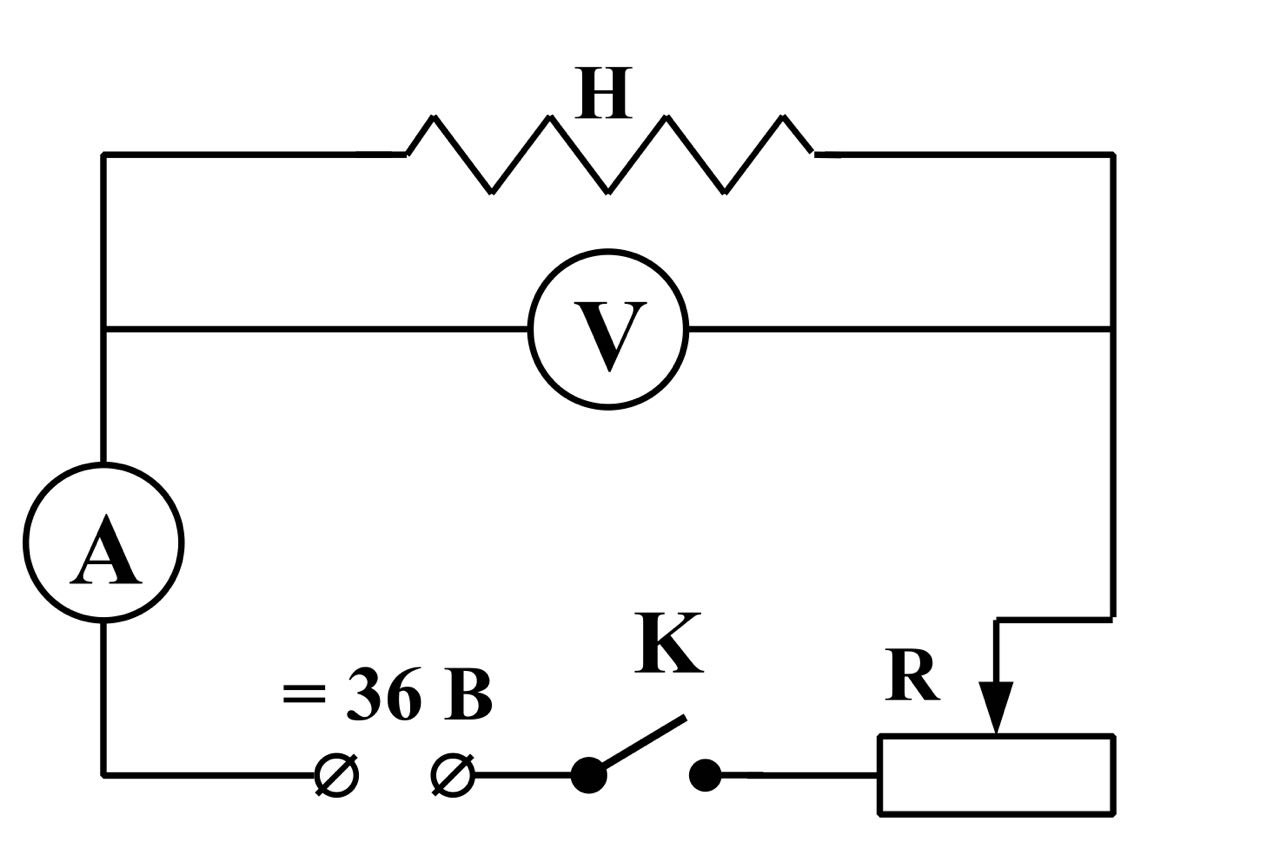
\includegraphics[scale=0.07]{2.1.4/schem.jpg}
		\caption{Схема включения нагревателя}
		\label{fig:schem_of_facility}
	\end{center}
\end{wrapfigure}

Установка состоит из калориметра с пенопластовой изоляцией, помещенного в ящик из многослойной клееной фанеры. Внутренние стенки калориметра выполнены из материала с высокой теплопроводностью. Надежность теплового контакта между телом и стенками обеспечивается их формой: они имеют форму усеченных конусов и плотно прилегают друг к другу. Для выталкивания образца служит винт в донышке внутренней стенки калориметра.

В стенку калориметра вмонтированы электронагреватель и термометр сопротивления. Схема включения нагревателя изображена на рисунке (\ref{fig:schem_of_facility}). Система реостатов позволяет установить нужную силу тока в цепи нагревателя. По амперметру и вольтметру определяется мощность, выделяемая током в нагревателе. Величина сопротивления термометра нагревателя  измеряется мостом постоянного тока.

\begin{figure}[h!]
	\begin{center}
		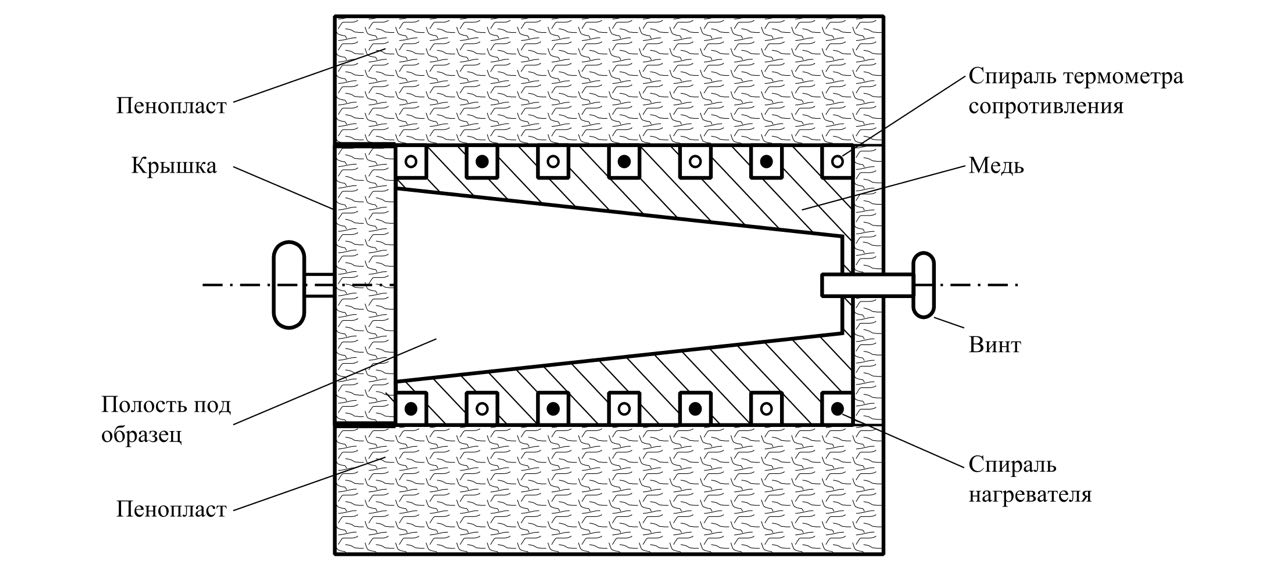
\includegraphics[scale=0.3]{2.1.4/ustfig.jpg}
		\caption{Устройство калориметра}
		\label{fig:Ris_of_facility}
	\end{center}
\end{figure}	

На рисунке (\ref{fig:Ris_of_facility}) изображено устройство калориметра.

Запишем также иные параметры экспериментальной установки:

\begin{table}[h!]
	\centering
	\begin{tabular}{|c|c|c|}
		\hline
		материал образца: & железо & алюминий        \\ \hline
		масса образца, г  & $813,12\pm 0,1$ & $294,2 \pm 0,1$ \\ \hline
	\end{tabular}
	\caption{Параметры исследуемых образцов}
	\label{tab:param_of_facility}
\end{table}

$$R_{0} = 17,84 \pm 0,01 \, \text{Ом}, \quad t_{0} = 24,4^{\circ} \pm 1 ^{\circ} C$$

$$ U = 36 \, \text{В}, \, I = 0,3 \, \text{А}, \, P = 10,8 \, \text{Вт} $$

\section{Измерения}

Снимем зависимость $R(t)$ для калориметра, а также для 2 исследуемых образцов. Данные занесем в таблицу (\ref{results_of_measuring_}).
	
\begin{table}[h]
    \begin{tabular}{|p{3cm}|p{3cm}|p{3cm}|p{3cm}|}
    \hline

\multicolumn{2}{|c|}{Калориметр с алюминиевым образцом} & \multicolumn{2}{|c|}{Калориметр с железным образцом}\\ \hline
R, Ом & t, c & R, Ом & t, c \\ \hline
17,95 & 0 & \multicolumn{2}{|c|}{---} \\ \hline
18,00 & 48 & 18,00 & 0 \\ \hline
18,05 & 108 & 18,05 & 62 \\ \hline
18,10 & 171 & 18,10 & 130 \\ \hline
18,15 & 236 & 18,15 & 202 \\ \hline
18,20 & 303 & 18,20 & 275 \\ \hline
18,25 & 373 & 18,25 & 351 \\ \hline
18,30 & 443 & 18,30 & 430 \\ \hline
18,35 & 514 & 18,35 & 510 \\ \hline
18,40 & 592 & 18,40 & 593 \\ \hline
18,45 & 669 & 18,45 & 679 \\ \hline
18,50 & 748 & 18,50 & 766 \\ \hline
18,55 & 830 & 18,55 & 856 \\ \hline

\multicolumn{4}{c}{} \\ \hline

\multicolumn{4}{|c|}{Пустой калориметр}\\ \hline
\multicolumn{2}{|l|}{R, Ом} & \multicolumn{2}{|l|}{t, с}  \\ \hline 
\multicolumn{2}{|l|}{17,95} & \multicolumn{2}{|l|}{0}  \\ \hline     
\multicolumn{2}{|l|}{18,00} & \multicolumn{2}{|l|}{40}  \\ \hline     
\multicolumn{2}{|l|}{18,05} & \multicolumn{2}{|l|}{87}  \\ \hline     
\multicolumn{2}{|l|}{18,10} & \multicolumn{2}{|l|}{135}  \\ \hline     
\multicolumn{2}{|l|}{18,15} & \multicolumn{2}{|l|}{184}  \\ \hline     
\multicolumn{2}{|l|}{18,20} & \multicolumn{2}{|l|}{235}  \\ \hline     
\multicolumn{2}{|l|}{18,25} & \multicolumn{2}{|l|}{288}  \\ \hline     
\multicolumn{2}{|l|}{18,30} & \multicolumn{2}{|l|}{342}  \\ \hline     
\multicolumn{2}{|l|}{18,35} & \multicolumn{2}{|l|}{397}  \\ \hline     
\multicolumn{2}{|l|}{18,40} & \multicolumn{2}{|l|}{454}  \\ \hline     
\multicolumn{2}{|l|}{18,45} & \multicolumn{2}{|l|}{513}  \\ \hline 

    \end{tabular}
    \caption {Результаты измерения сопротивления от времени нагрева}
    \label{results_of_measuring_}
\end{table}

\section{Обработка данных}

По полученым данным построим график зависимости $R(t)$.
	
\begin{figure}[h!]
	\begin{center}
		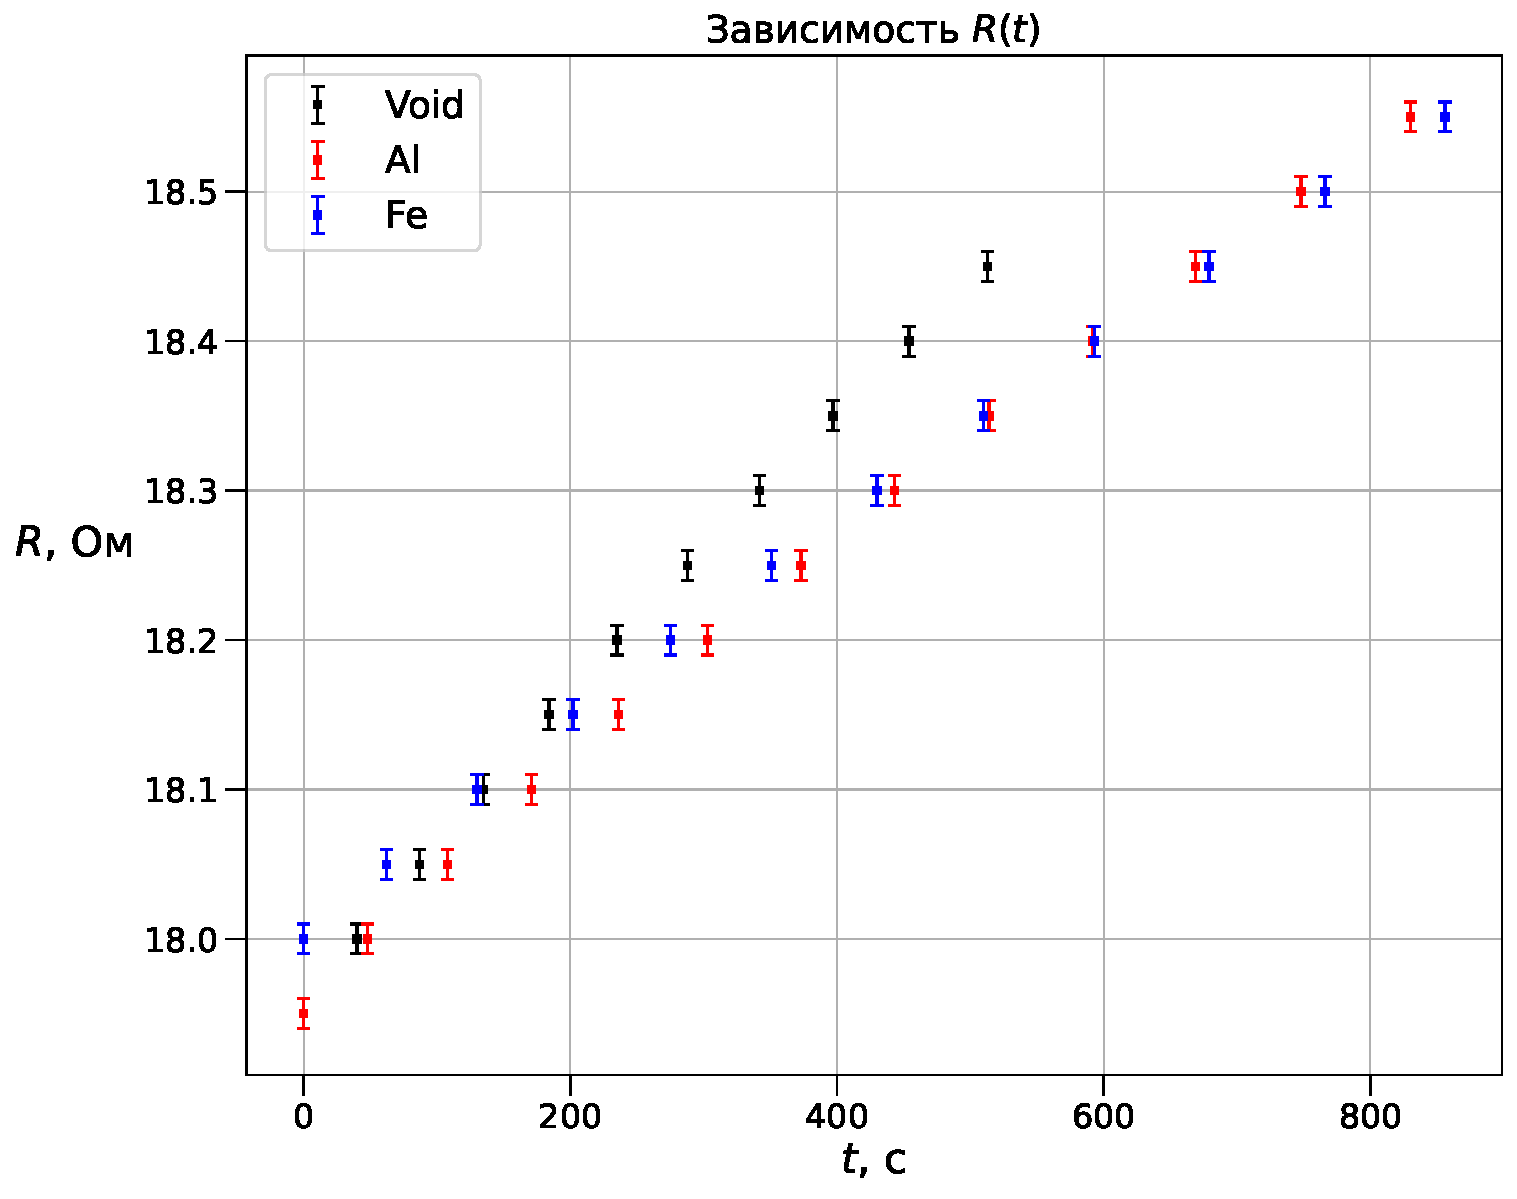
\includegraphics[scale=0.6]{2.1.4/R(t).pdf}
		\caption{График зависимости сопротивления от времени нагрева}
		\label{fig:results_of_measuring}
	\end{center}
\end{figure}

По полученным данным построим также графики зависимостей $\displaystyle \frac{dR}{dt} \left( R \right)$ для различных серий измерений, т.е. для калориметра и 2 исследуемых образцов. Данную зависимость построим с учетом формулы:

\begin{equation}
	\frac{dR}{dt} \left( R_{t_{1}} \right) = \frac{R_{t_{2}} - R_{t_{1}}}{t_{2} - t_{1}}
	\label{eq:derivates}
\end{equation}

Применив формулу (\ref{eq:derivates})  к данным таблицы (\ref{results_of_measuring_}), построим графики искомых зависимостей. График  изображен на рисунке (\ref{ris:dR_dt(r)_for_calorimetr}). 

\begin{figure}[H]
	\begin{center}
		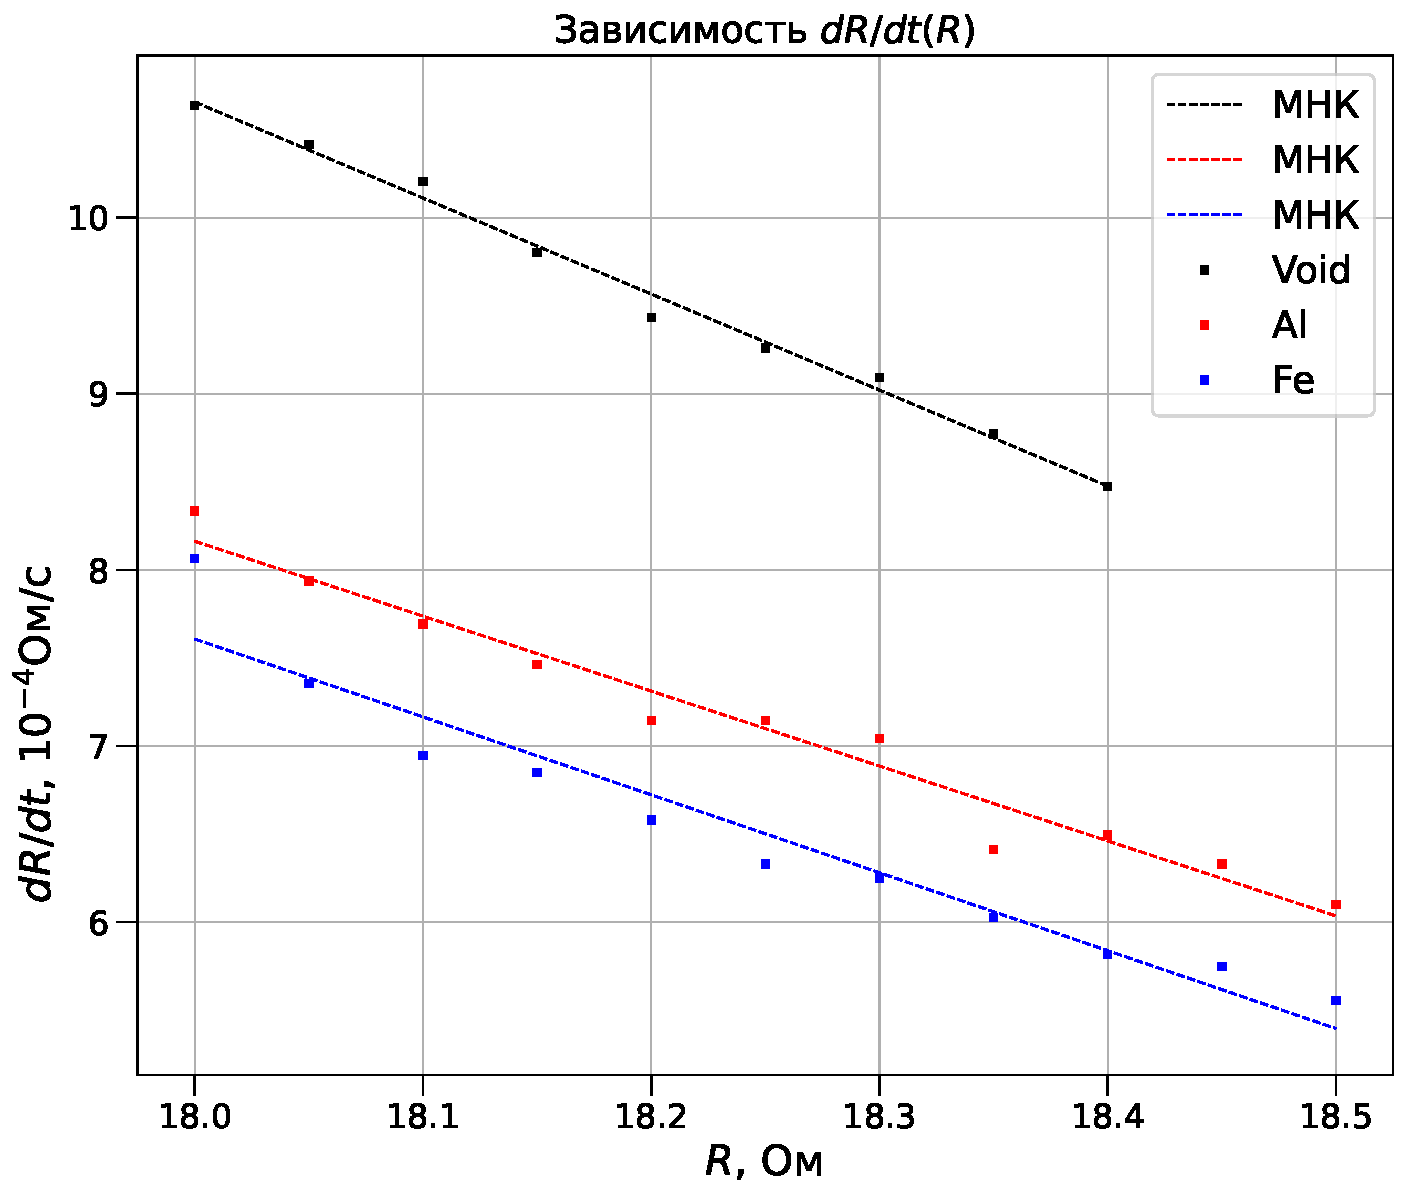
\includegraphics[scale=0.6]{2.1.4/dRdt.pdf}
		\caption{График зависимости $dR/dt$}
		\label{ris:dR_dt(r)_for_calorimetr}
	\end{center}
\end{figure}

Экстраполируя график для величин сопротивления при комнатной темпратуре, мы получаем следующие значения для теплоёмкости:
\begin{center}
$\displaystyle    C_0 = 650 \pm 32,5\ \frac{\mbox{Дж}}{\mbox{K}},\ \sigma_{C_0} = 5\%$
\break

$\displaystyle     C_{Al} = 246 \pm 12,4\  \frac{\mbox{Дж}}{\mbox{K}},\ \sigma_{C_{Al}} = 5\%$
\break

$\displaystyle     C_{Fe} = 309 \pm 15,7\  \frac{\mbox{Дж}}{\mbox{K}},\ \sigma_{C_{Fe}} = 5\%$
\break

\end{center}


Им соответствуют следующие удельные теплоёмкости:
\begin{center}

$\displaystyle     C^{\ m}_{Al} = 836 \pm 41,8\  \frac{\mbox{Дж}}{\mbox{K кг}},\ \sigma_{C^{\ m}_{Al}} = 5\%$
\break

$\displaystyle     C^{\ m}_{Fe} = 380 \pm 19,0\  \frac{\mbox{Дж}}{\mbox{K кг}},\ \sigma_{C^{\ m}_{Fe}} = 5\%$
\break

\end{center}

И молярные теплоёмкости:

\begin{center}

$\displaystyle     c_{Al} = 22,6 \pm 1,13\  \frac{\mbox{Дж}}{\mbox{K моль}},\ \sigma_{c_{Al}} = 5\%$
\break

$\displaystyle     c_{Fe} = 21,3 \pm 1,06\  \frac{\mbox{Дж}}{\mbox{K моль}},\ \sigma_{c_{Fe}} = 5\%$
\break

\end{center}


\end{document}
